%% ============================================================================
%%  Answer Locally, Verify Rarely
%%  IEEE conference paper (IEEEtran, two-column)
%%
%%  OVERLEAF SETUP
%%  --------------
%%  1. Upload this file, references.bib, and the figures/ folder.
%%  2. Menu -> Compiler -> pdfLaTeX.  Menu -> Main document -> main.tex.
%%  3. Compile twice (LaTeX -> BibTeX -> LaTeX) so citations resolve.
%%     Overleaf usually does this automatically.
%%
%%  FIGURES
%%  -------
%%  Every \includegraphics below is followed by a "REPLACE WITH" note naming
%%  exactly which diagram it is, so a cleaner redraw can be dropped in without
%%  guessing.  Keep the same file name and nothing else has to change.
%% ============================================================================

\documentclass[conference]{IEEEtran}
\IEEEoverridecommandlockouts

\usepackage{cite}
\usepackage{amsmath,amssymb}
\usepackage{graphicx}
\usepackage{booktabs}
\usepackage{url}
\usepackage[hidelinks]{hyperref}
\usepackage{textcomp}
\usepackage{xcolor}

\graphicspath{{figures/}}

\begin{document}

\title{Answer Locally, Verify Rarely: An Edge-Constrained\\
Supervised Cascade for Small-Model Mathematical Reasoning}

\author{
\IEEEauthorblockN{Author One, Author Two, Author Three}
\IEEEauthorblockA{\textit{Department Name} \\
\textit{Institution Name}\\
City, Country \\
email@institution.edu}
}

\maketitle

\begin{abstract}
Language models that are good at mathematical reasoning are large enough to require a
data centre. Running one on a phone or an ordinary laptop is not possible, and sending
every question to a cloud service costs money and moves private data off the device. We
ask whether a small model can do most of the work locally and request outside help only
rarely. We fine-tune \texttt{gemma-4-E2B-it} with 4-bit QLoRA on GSM8K, raising
exact-answer accuracy from $36.32\%$ to $55.88\%$ on the full 1{,}319-question test set
while reducing tokens read per question by a factor of eight. We then add an on-device
gate that escalates about $30\%$ of questions to a larger verifier, which marks the
reasoning, never sees the reference answer, and returns a short hint; the small model
then retries. The complete system reaches $68.46\%$, which is $93.9\%$ of the $72.93\%$
pass@3 ceiling, with $70\%$ of questions resolved entirely on-device. Two results are the
paper's contribution. First, the cascade must be \emph{stacked on} self-consistency rather
than substituted for it: run instead of free majority voting, no arm is statistically
distinguishable from it ($p=0.062$--$0.751$); layered on top, every arm is, and the gain
is exactly $+42$ answers at identical cost. Second, verifier capability is not monotonic
in size: a 9B verifier outperforms a 30B one on recall, false-reject rate and precision
simultaneously, at $1.0$\,s against $2.1$\,s per judgment. We do not claim a record; our
contribution is the trade-off curve between accuracy and how rarely the device asks for
help, together with the stacking result.
\end{abstract}

\begin{IEEEkeywords}
edge inference, model cascades, self-consistency, LLM verifiers, QLoRA, quantization,
mathematical reasoning, GSM8K
\end{IEEEkeywords}

% ============================================================================
\section{Introduction}
% ============================================================================

Models that score highly on mathematical reasoning benchmarks have hundreds of billions
of parameters. They run on specialised hardware in data centres, and using one means
sending the question over a network and paying per token.

Three costs follow, and all three recur for every question asked: a monetary cost that
never amortises, the departure of potentially sensitive data from the device, and a
dependency on network availability. Running a small model locally removes all three, but
small models are substantially worse at multi-step arithmetic reasoning. This paper is
about closing part of that gap without giving up the local-first property.

Our question is deliberately narrow: can a small model on the device do most of the work,
and escalate to a larger model rarely enough that the cost and privacy properties are
largely preserved? ``Rarely'' carries the argument. A cascade that escalates every
question is not a cascade; it is a slow proxy for the larger model. The design is only
meaningful if escalation is the exception, and we therefore report accuracy against
off-device tokens per question throughout.

\subsection{Contributions}

\begin{enumerate}
\item \textbf{A supervised cascade must be stacked on self-consistency, not substituted
for it.} Used in place of free majority voting, our cascade is not statistically
distinguishable from it. Layered on top --- vote first, escalate only the split votes ---
every configuration is, and the improvement is free, because the gate has already
generated the samples the vote requires.
\item \textbf{Verifier capability is not monotonic in parameter count.} Over a four-rung
ladder (2B self-verification, 9B, 30B-A3B, exact oracle) the 9B verifier dominates the
30B one on every measure taken.
\item \textbf{The most informative gate signal costs nothing when voting is already in
use.} Sample disagreement (AUC $0.840$) substantially outperforms the model's own
confidence ($0.715$), and a lexicographic tie-break on confidence reaches $0.869$ with no
tunable weight.
\end{enumerate}

\subsection{What we do not claim}

We do not claim state-of-the-art accuracy on GSM8K. TinyGSM~\cite{liu2023tinygsm} reports
$81.5\%$ with a 1.3B generator and a 1.3B trained verifier, and Qwen2.5-1.5B-Instruct is
reported at $73.2\%$ with no fine-tuning and no cascade~\cite{qwen2024qwen25}.
Section~\ref{sec:higher} addresses both directly. We also make no claim about reasoning
validity: our metric is the final answer only.

% ============================================================================
\section{Related Work}
% ============================================================================

\subsection{Small models on mathematical reasoning}

Cobbe \textit{et al.}~\cite{cobbe2021gsm8k} introduced GSM8K and, with it, the ancestor of
this work: training a separate verifier to rank sampled solutions, which allowed a 6B
model to outperform a 175B one. Their verifier selects among candidates; ours returns
feedback for a retry. Wei \textit{et al.}~\cite{wei2022cot} established chain-of-thought
prompting, the format of our training data. Hu \textit{et al.}~\cite{hu2022lora} and
Dettmers \textit{et al.}~\cite{dettmers2023qlora} contributed LoRA and QLoRA
respectively, which make our fine-tuning feasible on a single consumer GPU. Li
\textit{et al.}~\cite{li2025smallmodels} report that small models learn poorly from the
long reasoning traces produced by large models; our training data is short and
human-written, consistent with their recommendation.

\subsection{Test-time computation on a single model}

Wang \textit{et al.}~\cite{wang2023selfconsistency} introduced self-consistency --- sample
several solutions, take the majority. This is the most important reference for our work,
because it is free, requires no second model, and is the baseline our first design failed
to beat. Aggarwal \textit{et al.}~\cite{aggarwal2023adaptive} make the sampling adaptive,
stopping once agreement is reached; the instinct is the same as our gate's. Snell
\textit{et al.}~\cite{snell2024testtime} show that test-time computation can outperform a
model fourteen times larger, which is the general argument our design rests on. A recent
analysis~\cite{selfconsistency2025edge} reports that self-consistency's benefit is
diminishing on newer models; we do not observe that here, where voting yields a
statistically solid $+3.18$ points.

\subsection{Cascades and routing}

FrugalGPT~\cite{chen2023frugalgpt} is the canonical cost-saving cascade: attempt with a
cheap model, escalate when a scorer judges the output weak, with reported cost reductions
up to $98\%$. One structural difference matters for cost accounting: in FrugalGPT the
expensive model \emph{answers}; in ours it only \emph{judges}. The off-device payload is
therefore a short verdict rather than a full solution.

Gupta \textit{et al.}~\cite{gupta2024cascades} is the closest published work to our gate,
deferring on token-level uncertainty and reporting that response length is a biased
signal. We measure the same effect: length is our weakest gate at AUC $0.676$. Zellinger
\textit{et al.}~\cite{zellinger2025abstention} add early abstention,
RouteLLM~\cite{ong2024routellm} learns a router, and Big Little
Decoder~\cite{kim2023bild} switches models mid-sequence. None returns feedback for a
retry.

\subsection{Model-based verification}

Zheng \textit{et al.}~\cite{zheng2023judge} established LLM-as-a-judge, reporting over
$80\%$ agreement with human judges, and documented self-enhancement bias --- models favour
their own outputs. That bias predicts our measured failure of 2B self-verification
(Section~\ref{sec:ladder}). Lightman \textit{et al.}~\cite{lightman2023verify} show
process supervision outperforms outcome supervision; we verify whole solutions at once,
which is cheaper and weaker, and their result describes what we leave unexploited. ``Not
All Votes Count!''~\cite{notallvotes2024} weights votes by verifier confidence, reporting
up to $+18\%$ on GSM8K; this is the nearest analogue to our stacking result, reached by a
different mechanism.

\subsection{Negative results that motivate our design}

Huang \textit{et al.}~\cite{huang2024selfcorrect} report that language models cannot
reliably self-correct reasoning without external information. Our blind-retry control
replicates this on a model roughly two orders of magnitude smaller: accuracy falls from
$55.88\%$ to $49.89\%$. Zhang \textit{et al.}~\cite{zhang2024strongverifiers} is the
closest work to our verifier-strength question, comparing two verifier scales; we extend
the comparison to four rungs and find the relationship is not monotonic.
Self-Refine~\cite{madaan2023selfrefine} and Reflexion~\cite{shinn2023reflexion} report
gains from iterative self-criticism on much larger models; the tension
with~\cite{huang2024selfcorrect} is unresolved in the literature, and our result falls on
Huang's side.

\subsection{Inference on constrained hardware}

Lu \textit{et al.}~\cite{lu2024smallsurvey} survey small language models, and a recent
benchmark of over 60 edge-deployable models~\cite{unified2026deployment} reports that
compressed sub-7B models retain roughly $90$--$95\%$ of their quality. Bondarenko
\textit{et al.}~\cite{bondarenko2026edge} is concurrent work on efficient edge reasoning
that optimises the model itself; our approach holds the model fixed and adds a verifier,
so the two are complementary.

\subsection{Systems reporting higher accuracy}
\label{sec:higher}

Two results exceed ours on GSM8K, and we address them directly.

\textbf{TinyGSM}~\cite{liu2023tinygsm} reports $81.5\%$ using a 1.3B generator and a 1.3B
trained verifier. The protocol differs in ways that matter for a cost argument: training
uses 12.3M synthetic problems generated by GPT-3.5 (roughly $1{,}600\times$ our data),
solutions are executed Python rather than natural language, the verifier is trained rather
than prompted, and the headline metric is \emph{verify48@1} --- 48 sampled generations per
question, all verifier-scored. That last figure is $16\times$ our local generation budget,
on precisely the axis this paper argues about. We also note plainly that their
fine-tuning-only model reaches $68.2\%$, above our $55.88\%$, which we attribute to the
synthetic training corpus rather than to architecture.

\textbf{Qwen2.5-1.5B-Instruct} is reported at $73.2\%$ (4-shot)~\cite{qwen2024qwen25} ---
fewer parameters than our base model, no fine-tuning, no cascade, above our complete
system.

A distinction is worth making, because ``smaller model'' is ambiguous. Parameter count is
not what determines whether a model runs on a device; memory is. Both systems above are
reported at 16-bit precision, whereas we deploy at 4-bit (Table~\ref{tab:footprint}).

\begin{table}[t]
\caption{Deployment footprint at the precision each system reports.}
\label{tab:footprint}
\centering
\begin{tabular}{@{}lccr@{}}
\toprule
System & Parameters & Bits & Memory \\
\midrule
TinyGSM (both models resident) & 1.3B + 1.3B & 16 & 4.84\,GB \\
Qwen2.5-1.5B-Instruct & 1.54B & 16 & 2.88\,GB \\
\textbf{This work, as deployed} & 5.12B stored & \textbf{4} & \textbf{2.39\,GB} \\
\bottomrule
\end{tabular}
\end{table}

On the axis of interest, our solver is the smallest of the three despite the largest
parameter count. Two qualifications: those systems could be quantized as well --- a 4-bit
Qwen2.5-1.5B would be approximately $0.72$\,GB --- but no published score exists in that
form and quantization costs accuracy; and we assume 16-bit for their figures, as neither
reports quantized results. The fair summary is that they report higher accuracy with fewer
parameters, but not with a smaller deployment footprint. Our claims are paired comparisons
on a single base model, and the mechanism rather than the absolute score is the
contribution.

% ============================================================================
\section{Method}
% ============================================================================

% ---------------------------------------------------------------------------
% FIGURE 1
% REPLACE WITH: the cleaned SYSTEM ARCHITECTURE diagram.
%   Current source : reports/figures/technical/fig1_system_architecture.png
%   Plain-language twin: reports/figures/fig1_system_architecture.png
%   Shows: device boundary (solver + vote + gate) vs. off-device verifier,
%          the escalation arrow, and the hint returning.
%   Must still show: the verifier NEVER receives the reference answer.
%   Single column. Save the redraw as figures/fig1_system_architecture.pdf
%   (or .png) and nothing below has to change.
% ---------------------------------------------------------------------------
\begin{figure}[t]
\centering
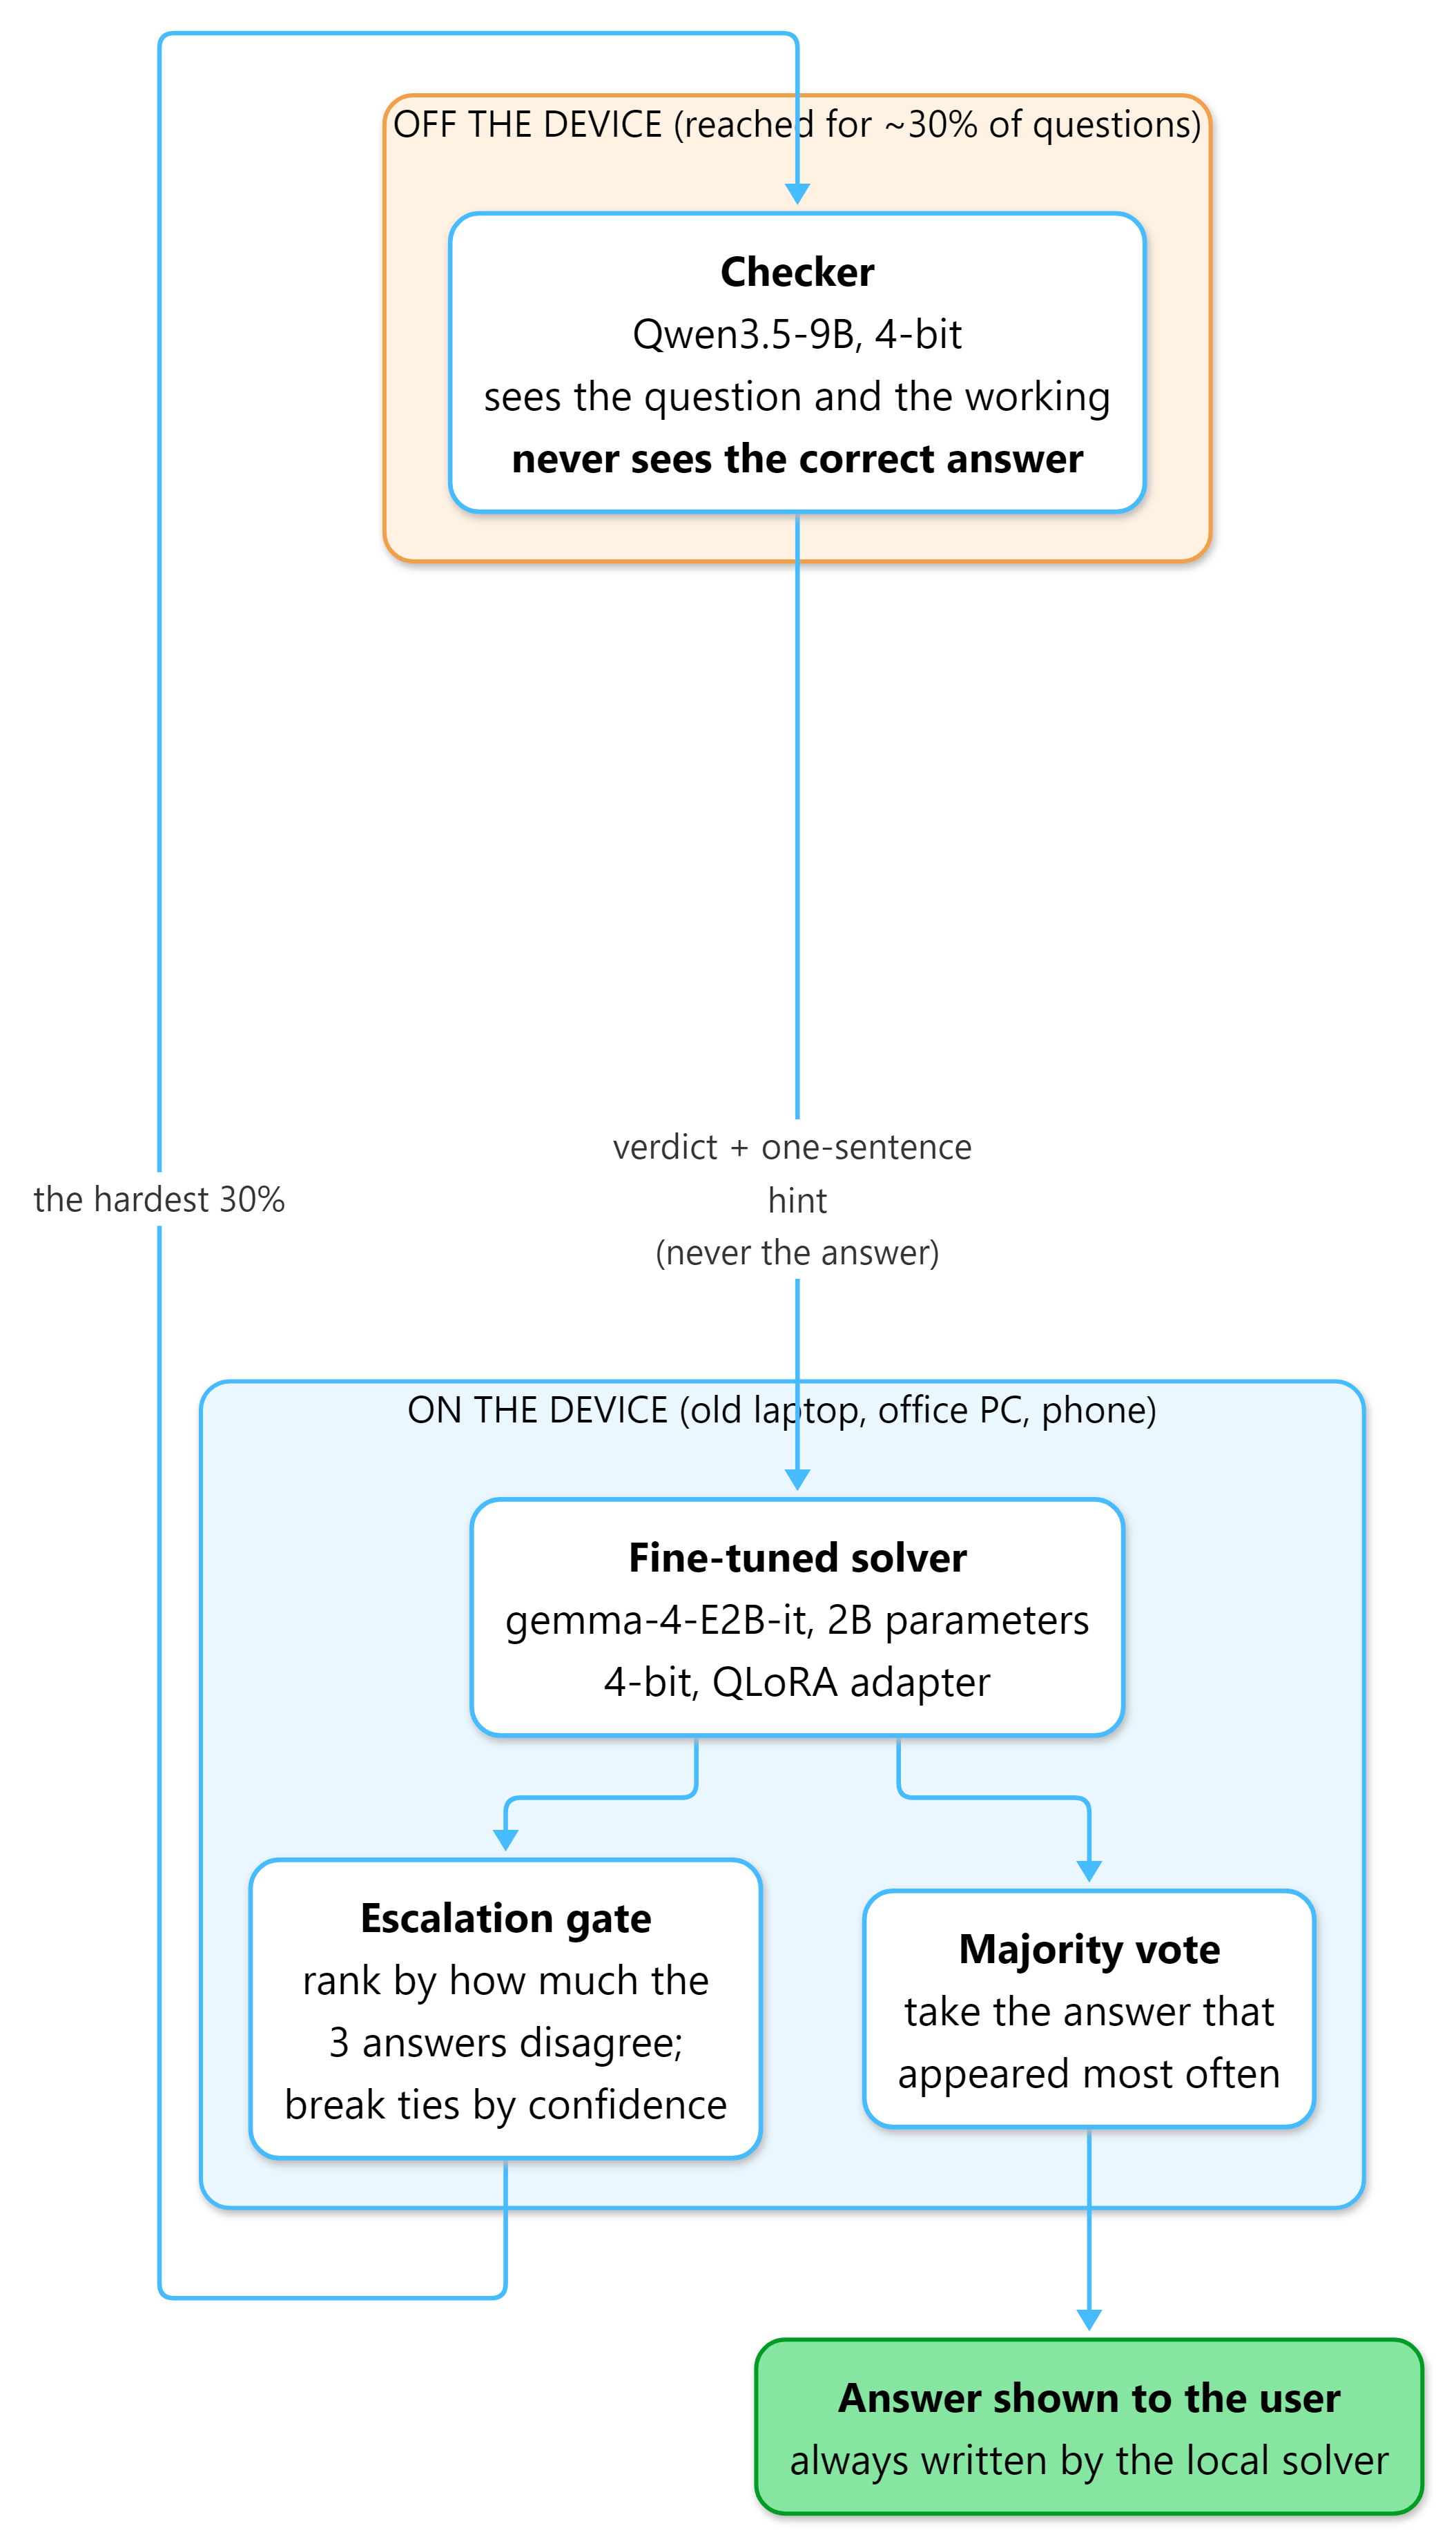
\includegraphics[width=\columnwidth]{fig1_system_architecture.png}
\caption{System architecture. Everything inside the device boundary runs locally. The
supervisor is contacted only for questions the gate selects, and never receives the
reference answer.}
\label{fig:arch}
\end{figure}

\subsection{Dataset}

We use the official GSM8K release (\texttt{openai/gsm8k}, configuration \texttt{main}):
7{,}473 training and 1{,}319 test problems. Every reported number is measured on the
complete test split.

No filtering, deduplication, or cleaning is applied; all 7{,}473 training problems are
used, and the calculator annotations native to the dataset are retained. Each example is
formatted into the model's chat layout, with the reference solution terminated by the
dataset's \verb|#### N| marker. Sequences are truncated at 1{,}024 tokens rather than
dropped.

\textbf{Answer extraction and matching.} We extract the text following the final
\verb|####| marker, falling back to the last numeric token when no marker is present.
Before comparison, both strings have \verb|$| and \verb|%| removed, trailing periods and
commas stripped, the first numeric token taken, fractions evaluated, and the result
converted to an exact rational. Thus \texttt{72.0}, \texttt{\$1,200} and \texttt{1/2}
match \texttt{72}, \texttt{1200} and \texttt{0.5}. There is no partial credit and no human
adjudication. This logic is covered by automated tests, and the fine-tuned model produced
an extractable answer on 1{,}318 of 1{,}319 test problems.

\subsection{Quantization and fine-tuning}

The base model is \texttt{google/gemma-4-E2B-it}, a multimodal model with 5.12B stored
parameters (4.65B in the text tower) across 35 layers, of which 20 share key/value
projections with earlier layers.

We load in 4-bit NF4 with double quantization and bfloat16 compute, then attach LoRA
adapters (rank 16, $\alpha$ 32, dropout 0.05) to all seven projections in each
language-model layer. The KV-sharing above means 15 layers admit seven attachment points
and 20 admit five, giving 205 adapted modules rather than the expected 245, and
$24{,}158{,}208$ trainable parameters --- $0.47\%$ of the model --- in a 97\,MB adapter.
Loss is computed on completion tokens only; prompt and padding positions are masked.

Training runs for 3 epochs (1{,}404 optimizer steps) at learning rate $2\times10^{-4}$
with a cosine schedule and 50 warm-up steps, batch size 1 with 16-step gradient
accumulation. Training loss falls from $2.317$ to $0.250$ and token accuracy rises from
$0.687$ to $0.923$. Epoch-end evaluation is disabled: it requested an additional 4.38\,GB
on a 16\,GB card and terminated the run at step 936, from which we resumed at step 900. We
evaluate after training by generating and grading all 1{,}319 test answers instead.

\subsection{The escalation gate}

% ---------------------------------------------------------------------------
% FIGURE 2
% REPLACE WITH: the cleaned ESCALATION GATE diagram.
%   Current source : reports/figures/technical/fig4_the_escalation_gate.png
%   Plain-language twin: reports/figures/fig4_the_escalation_gate.png
%   Shows: the three disagreement buckets (427 / 400 / 492) and the confidence
%          tie-break operating INSIDE the 492 only.
%   Must still show: confidence can never outrank disagreement.
%   Single column. Save as figures/fig4_the_escalation_gate.pdf (or .png).
% ---------------------------------------------------------------------------
\begin{figure}[t]
\centering
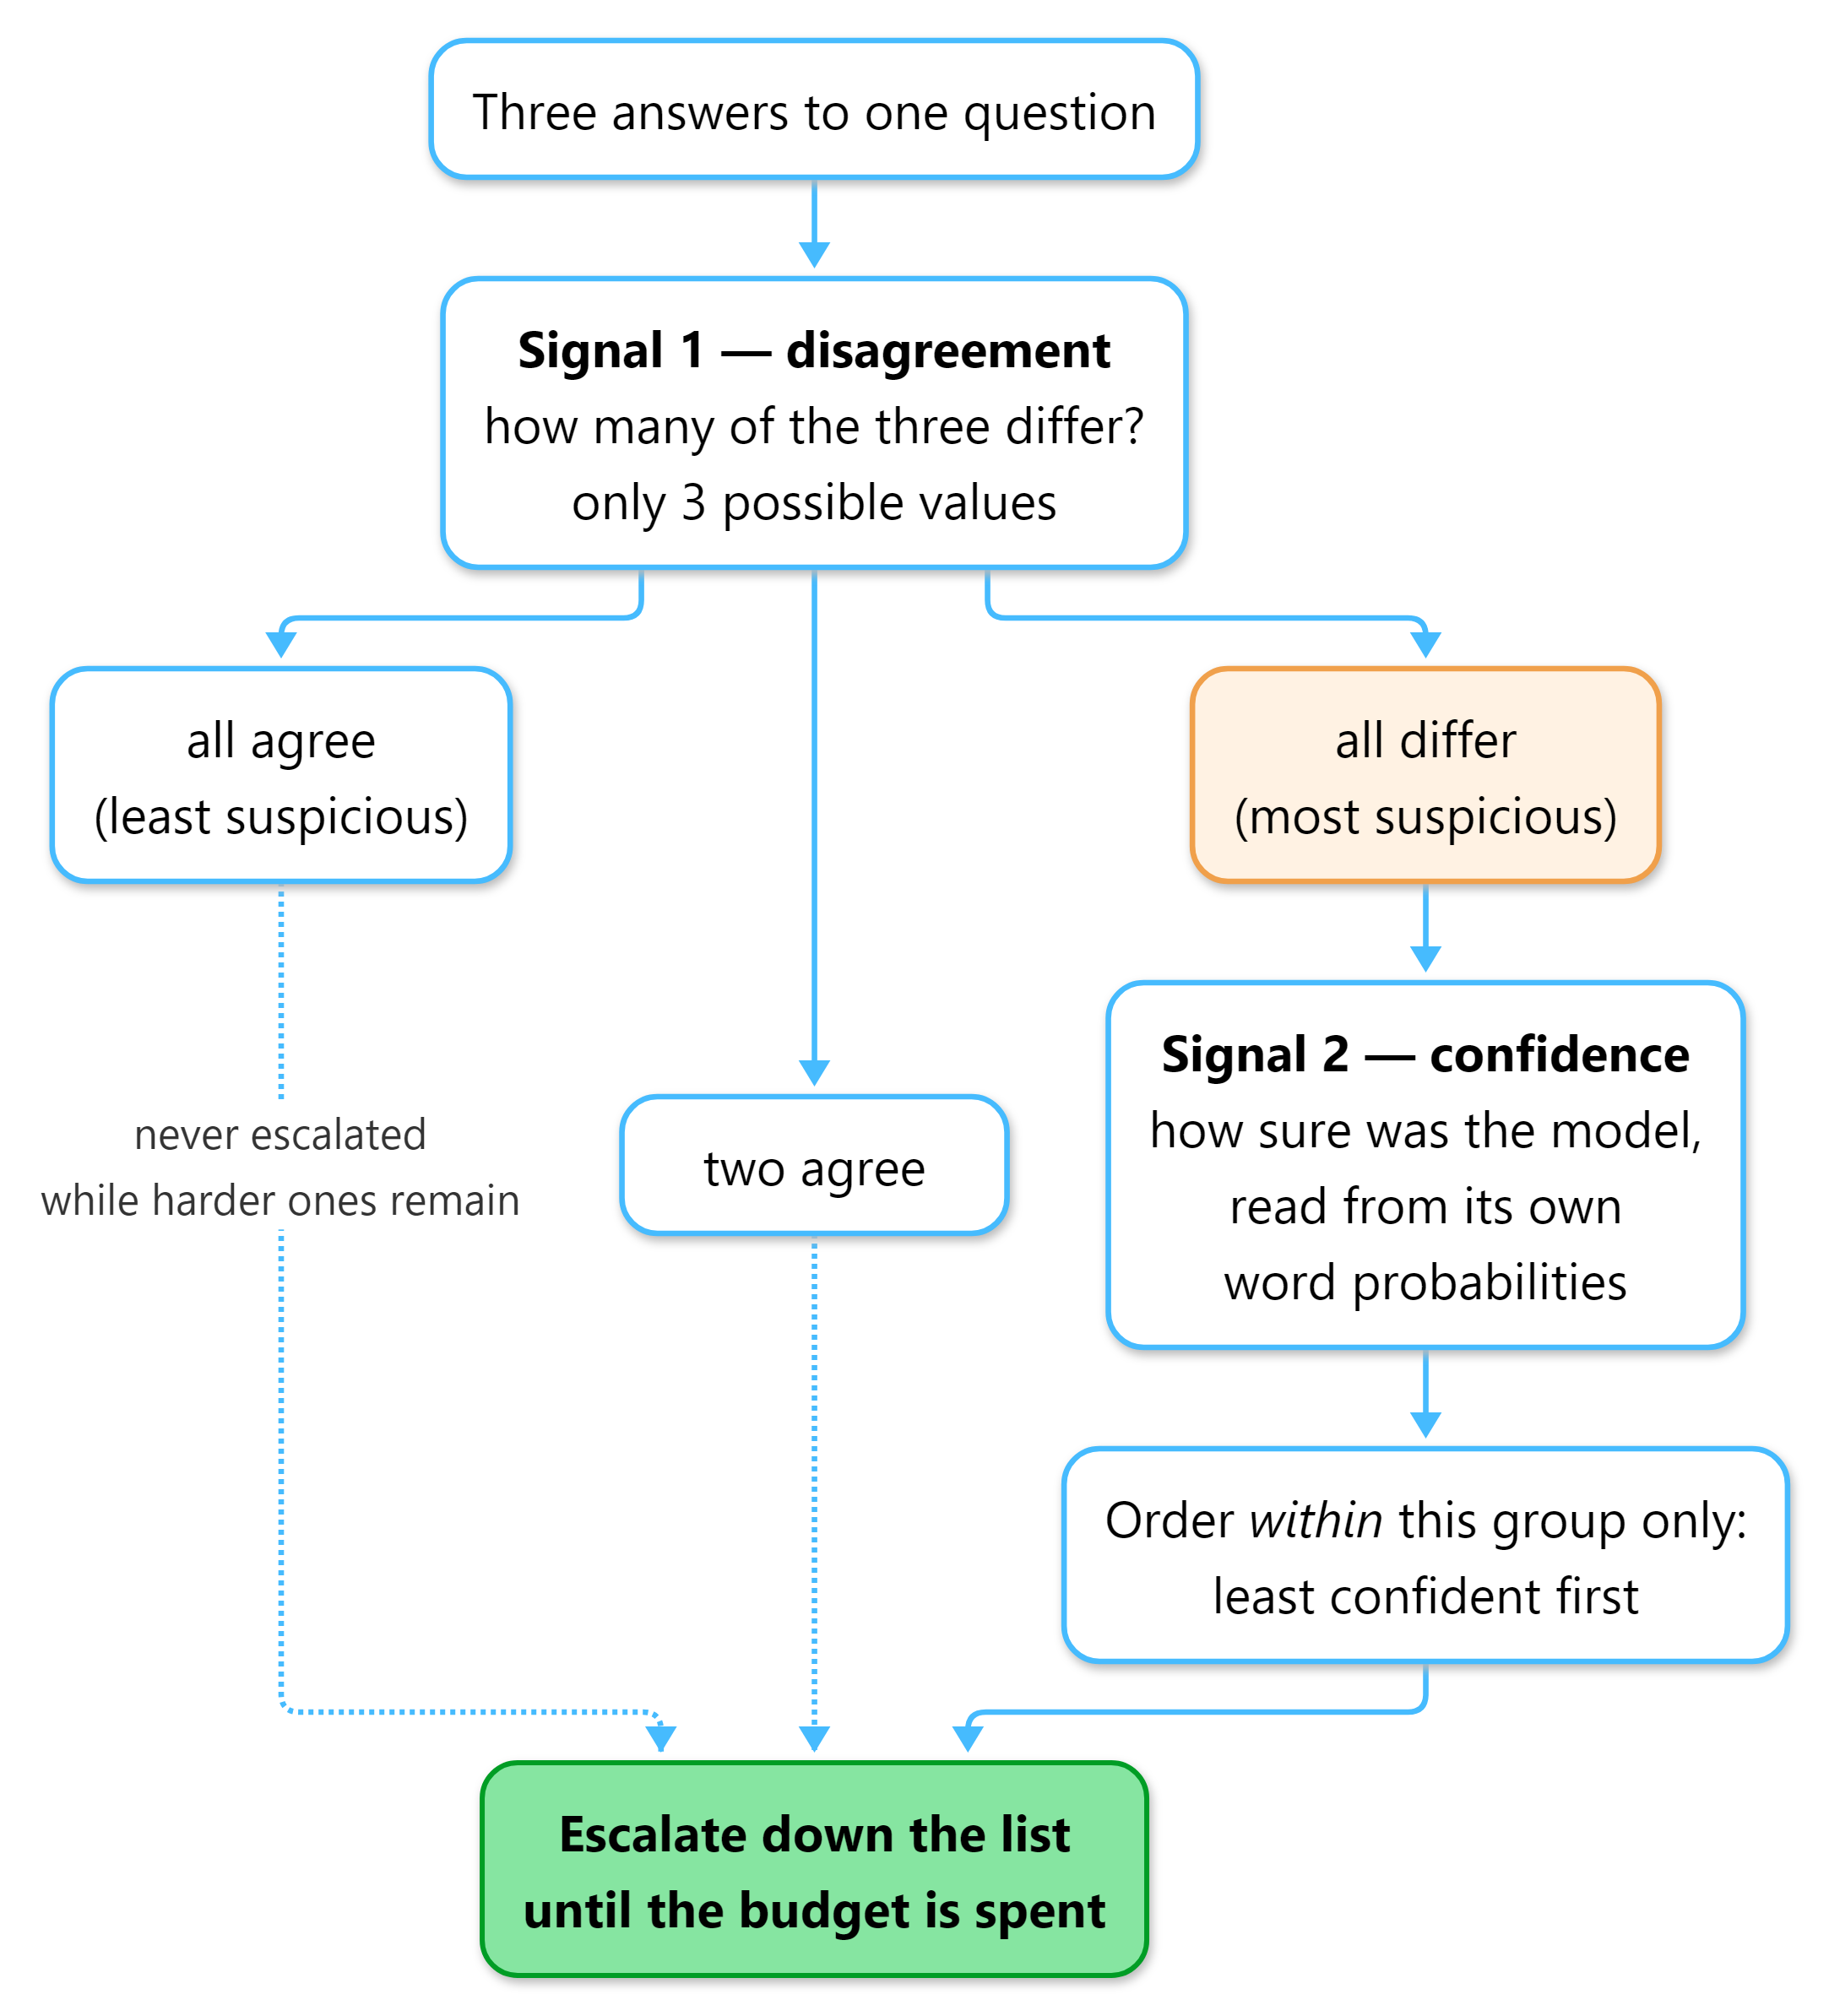
\includegraphics[width=\columnwidth]{fig4_the_escalation_gate.png}
\caption{The combined gate. Confidence reorders questions within a tied disagreement group
but can never outrank the primary signal, so no weight requires tuning.}
\label{fig:gate}
\end{figure}

The gate ranks questions by an on-device signal and escalates the top fraction under a
fixed budget. We evaluate four signals: response length, final-answer log-probability,
disagreement across $k=3$ samples, and disagreement with confidence as a lexicographic
tie-break.

Two properties are worth stating. First, with three samples disagreement admits only three
values, partitioning the test set into $427/400/492$ questions. The only escalation rate
the gate genuinely expresses is therefore $37.3\%$ (492 questions); a $30\%$ budget cuts
inside the tied group and the implementation breaks ties by index. We report both.

Second, the tie-break is strictly subordinate. Confidence is compressed inside the
smallest gap between primary values and can never reorder them. Permitting confidence to
outweigh disagreement scored \emph{worse} than disagreement alone. Because the combination
has no weight parameter, there is no quantity that could have been tuned on test data.

\subsection{The supervisor}

The supervisor receives the question and the candidate solution, and returns a verdict
with an optional hint. It never receives the reference answer; this is enforced at the
prompt boundary and asserted by a test, and any \verb|####| line in its reply is stripped
before the solver sees it.

Hint content is treated as a measured variable rather than a design choice, since hint
length is off-device output tokens: \textbf{L0} is the bare rejection ($\approx$12
tokens), \textbf{L1} adds a pointer naming the step that failed ($\approx$30), and
\textbf{L2} adds a correction stating the right interpretation ($\approx$57).

Supervisors are served as GGUF through \texttt{llama-server} rather than through
\texttt{transformers}. A 30B mixture-of-experts model would require quantizing from
$\sim$60\,GB of fp16 weights and would still not fit; the GGUF is 17.5\,GB and offloads
experts to system RAM. This also makes swapping verifiers a server restart, which is what
makes the four-rung ladder affordable.

\textbf{Safety properties.} An unparseable reply is treated as an \emph{accept}, never a
reject: the cascade must not manufacture rejections from its own defects. The corollary is
that ambiguity becomes silent approval, so empty and truncated replies are converted to
errors at the provider boundary, and the run aborts after a threshold of consecutive
failures rather than approving the remainder.

\subsection{Verdict caching as an experimental control}
\label{sec:cache}

Verdicts are cached, content-addressed on \textit{provider} $|$ \textit{model} $|$
\textit{system prompt} $|$ \textit{question} $|$ \textit{candidate answer}. The candidate
text must be in the key, since attempt 2 concerns a different solution to the same
question.

This is a validity mechanism, not an optimisation. The supervisor is not bit-reproducible
--- the same prompt and model at temperature 0 produced false-reject rates of $0.500$ and
$0.417$ in two runs --- so independently re-judging attempt 1 per arm would cause the
L0/L1/L2 arms to reject \emph{different} sets, confounding hint content with which
questions happened to be retried. Caching makes ``all arms reject the same set''
structural. Measured: 396 of 396 attempt-1 verdicts replayed identically across runs made
a day apart.

\subsection{The cascade, and stacking}
\label{sec:stacking}

% ---------------------------------------------------------------------------
% FIGURE 3  *** SPANS BOTH COLUMNS -- the most important figure in the paper ***
% REPLACE WITH: the cleaned PER-QUESTION DATA FLOW diagram.
%   Current source : reports/figures/technical/fig2_per_question_data_flow.png
%   Plain-language twin: reports/figures/fig2_per_question_data_flow.png
%   Shows the full test set flowing through, with these MEASURED counts:
%     1,319 questions -> 827 settled by vote / 492 split
%     -> 396 escalated (30% budget) + 96 left alone
%     -> 923 (70%) never leave the device
%     -> verifier rejects 332 -> retry -> accepts 85 -> 247 final unchecked try
%     -> 903 right, 416 wrong
%   Every one of those numbers is measured; do not round or alter them.
%   Full width (figure*). Save as figures/fig2_per_question_data_flow.pdf.
% ---------------------------------------------------------------------------
\begin{figure*}[t]
\centering
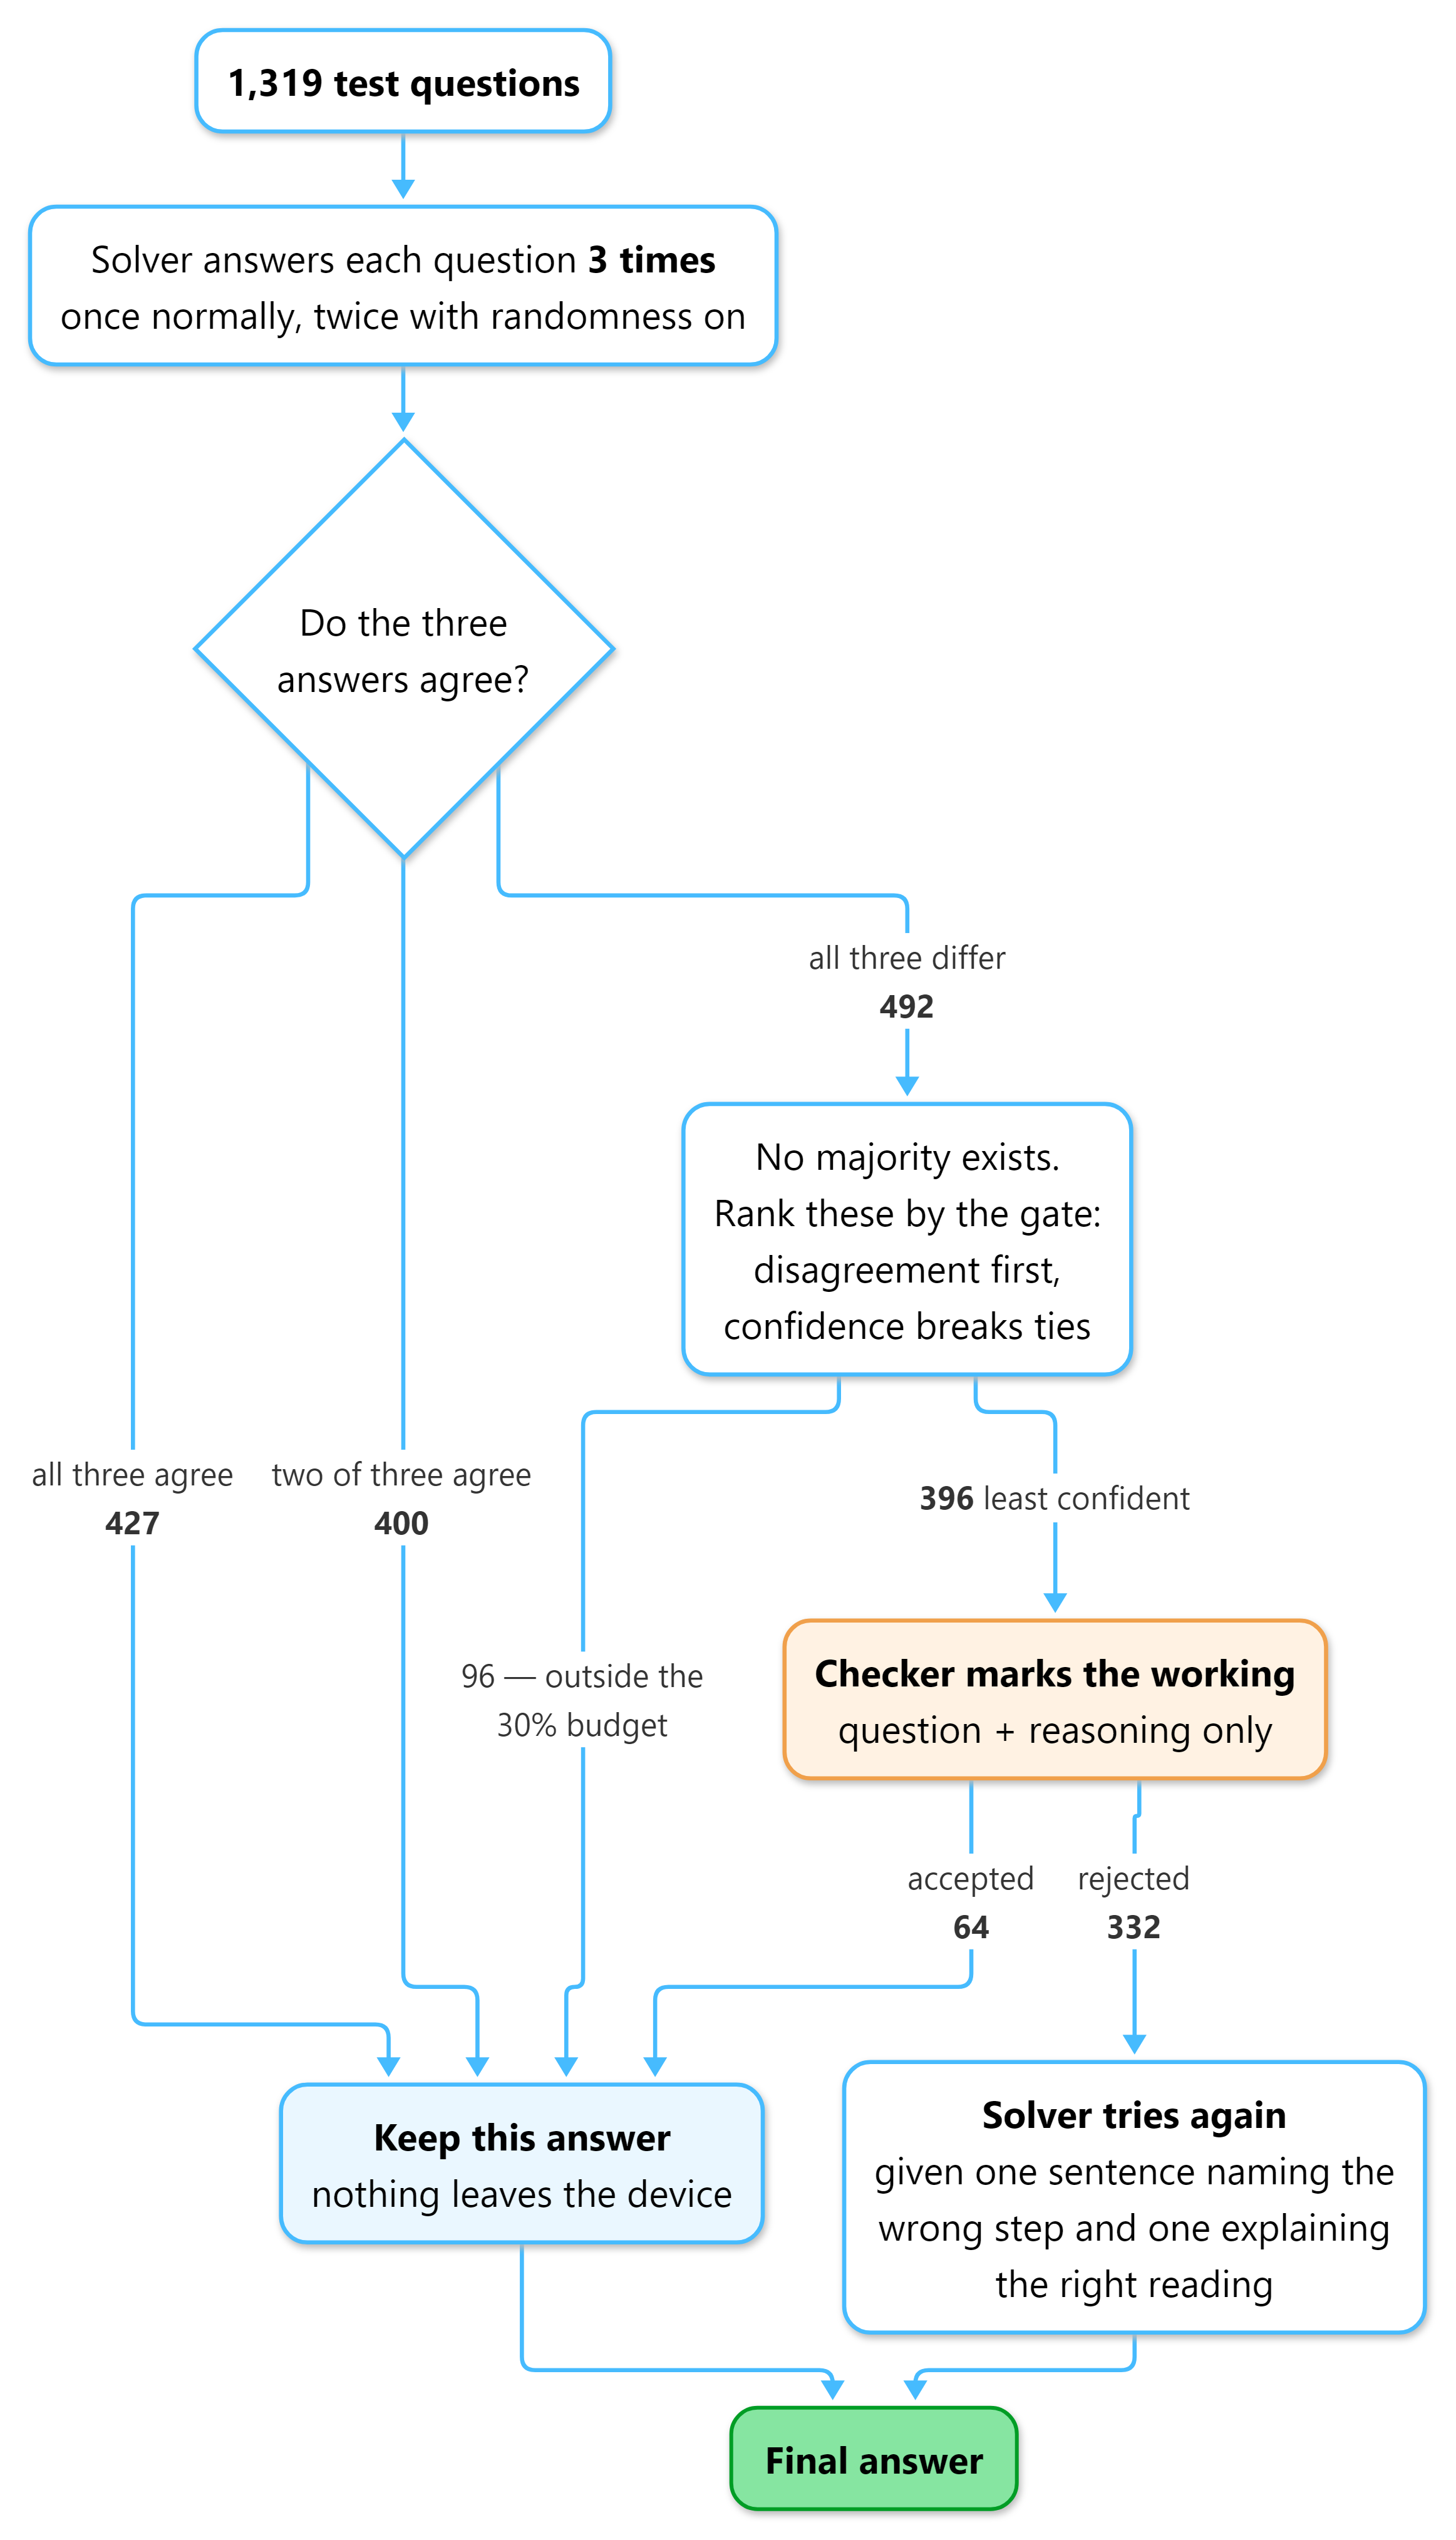
\includegraphics[width=0.82\textwidth]{fig2_per_question_data_flow.png}
\caption{Per-question data flow across the full GSM8K test set ($n=1{,}319$). All counts
are measured. 923 questions ($70\%$) are resolved entirely on-device.}
\label{fig:flow}
\end{figure*}

The complete system proceeds as follows. The solver generates three samples. Majority
voting resolves the 827 questions where a majority exists. The gate escalates 396 of the
remaining 492 under the $30\%$ budget; the other 96 retain their first attempt. The
supervisor rejects 332 of the 396; after the retry it accepts 85, and the remaining 247
receive one final unchecked attempt.

The stacking rule is: \emph{take the majority vote first, and use the cascade's output
only where the vote was split.} This is free. The gate has already generated the three
samples the vote requires --- it needs them to measure disagreement --- and the un-stacked
configuration simply discards them.

% ---------------------------------------------------------------------------
% FIGURE 4
% REPLACE WITH: the cleaned "WHY STACKING WORKS" diagram.
%   Current source : reports/figures/technical/fig3_why_stacking_works.png
%   Plain-language twin: reports/figures/fig3_why_stacking_works.png
%   Shows: voting repairs only the two-agree bucket (81 changes); the cascade
%          operates only on the all-differ bucket. The sets are DISJOINT --
%          that disjointness is the whole point of the figure.
%   Single column, wide and short. Save as figures/fig3_why_stacking_works.pdf.
% ---------------------------------------------------------------------------
\begin{figure}[t]
\centering
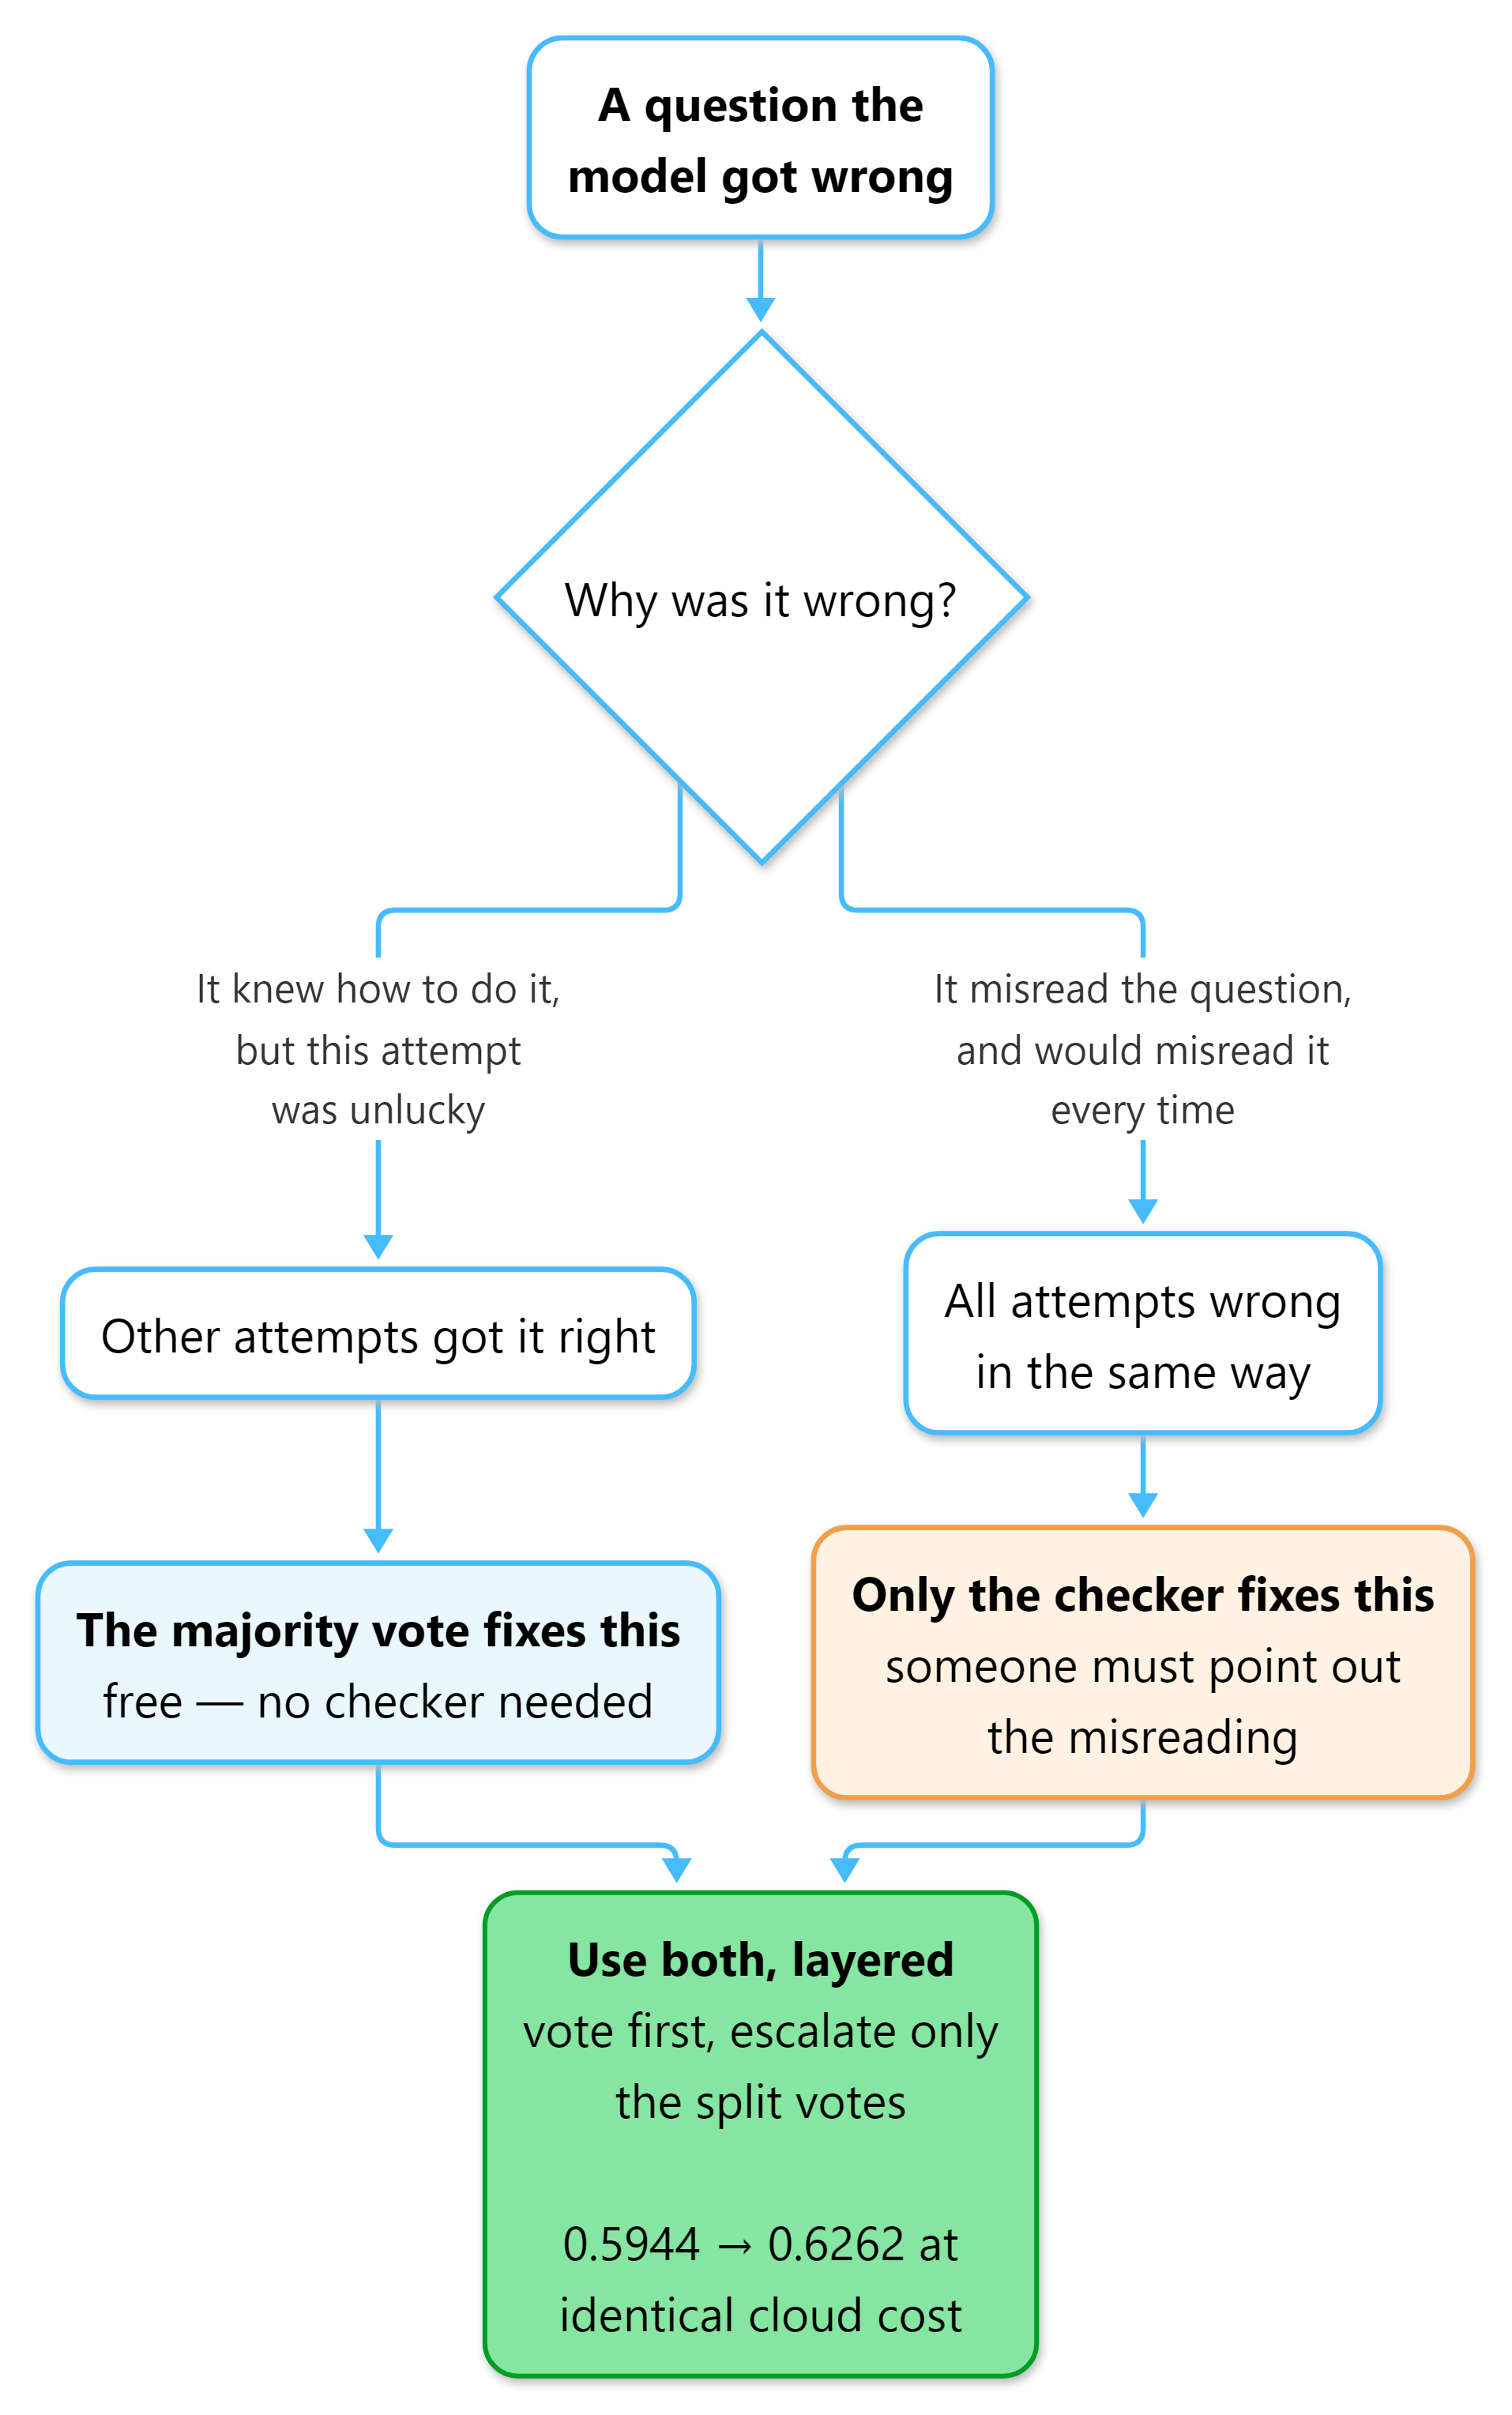
\includegraphics[width=\columnwidth]{fig3_why_stacking_works.png}
\caption{The two repair mechanisms operate on disjoint question sets, which is why their
gains add without interaction.}
\label{fig:stack}
\end{figure}

The gain is structural rather than incidental. Voting can only alter answers in the
two-agree/one-differs bucket, where it changes 81; the cascade operates only on the
all-differ bucket. The sets are disjoint, so the gains add without interaction --- which is
why the improvement is \emph{exactly} $+42$ for every arm (Section~\ref{sec:full}).

% ============================================================================
\section{Experimental Setup}
% ============================================================================

All experiments run on one workstation: NVIDIA RTX 4080 SUPER (16\,GB, driver 560.94),
32\,GB system RAM, Windows 11, Python 3.11.9, PyTorch 2.6.0+cu124, transformers 5.8.1,
peft 0.19.1, bitsandbytes 0.49.2, llama.cpp build b10453. Every model, supervisor
included, runs locally; no cloud service was used for any reported number.

Attempt 1 is greedy (temperature 0, $\leq$512 new tokens) with repetition penalty 1.15; we
note that this makes it greedy-with-penalty rather than pure argmax. Additional samples and
retries use temperature 0.7, with \texttt{top\_p} and \texttt{top\_k} left at library
defaults. Attempt 1 is generated once and reused across all arms; it was verified
byte-identical on a 20-example resample.

The untrained baseline is evaluated 8-shot, using the first eight training problems fixed
across all test questions. This is deliberate: prompted with a bare question the base model
scores $1.5\%$ and fails to produce an extractable answer on 566 of 1{,}319 problems, so a
zero-shot baseline would materially overstate the fine-tuning gain.

The supervisor prompt was calibrated on 150 \emph{training} problems. An earlier prompt was
calibrated on test problems; on discovering this we repeated the comparison on held-out
training data, where the original prompt proved net harmful ($-3.2$ expected answers per
150) against the adopted prompt ($+2.6$). We report the procedure rather than only the
outcome.

% ============================================================================
\section{Results}
% ============================================================================

\subsection{Fine-tuning}

\begin{table}[t]
\caption{Fine-tuning, full GSM8K test set ($n=1{,}319$).}
\label{tab:finetune}
\centering
\small
\begin{tabular}{@{}lrrrrr@{}}
\toprule
Condition & Corr. & Acc. & Prompt & Gen. & Total \\
\midrule
Base model, 8-shot & 479 & $36.32\%$ & 1617.7 & 120.6 & 1738.3 \\
\textbf{QLoRA, 0-shot} & \textbf{737} & $\mathbf{55.88\%}$ & \textbf{87.7} & 125.9 & \textbf{213.5} \\
\bottomrule
\end{tabular}
\end{table}

$+19.56$ points at $12.3\%$ of the token cost. The token reduction should be stated
carefully: the fine-tuned model is not more concise --- it generates slightly more
($125.9$ against $120.6$). The saving is entirely on the input side, from eliminating the
eight in-context exemplars.

\subsection{Free baselines and the ceiling}
\label{sec:free}

\begin{table}[t]
\caption{Configurations requiring no second model.}
\label{tab:free}
\centering
\small
\begin{tabular}{@{}lrrc@{}}
\toprule
Condition & Correct & Accuracy & Off-device cost \\
\midrule
Fine-tuned, single sample & 737 & $55.88\%$ & 0 \\
Blind retry, take last & 658 & $\mathbf{49.89\%}$ & 0 \\
Self-consistency@3 & 779 & $\mathbf{59.06\%}$ & 0 \\
pass@3 ceiling & 962 & $\mathbf{72.93\%}$ & 0 \\
\bottomrule
\end{tabular}
\end{table}

Three observations. \textbf{Blind retry is actively harmful}, costing 6 points: on one
sample it repaired 141 of 582 wrong answers while breaking 229 of 737 correct ones.
Resampling is asymmetric and hostile, which is the principal reason verifier
\emph{precision} matters more than recall in this design. \textbf{Self-consistency is a
strong free baseline} at $59.06\%$. And \textbf{$72.93\%$ is a hard ceiling}: an answer the
solver never produces cannot be recovered by any verifier, so all subsequent results should
be read against the $55.88$--$72.93\%$ band.

\subsection{Gate quality}

\begin{table}[t]
\caption{Gate signal quality (AUC) on the full test set.}
\label{tab:auc}
\centering
\small
\begin{tabular}{@{}lcl@{}}
\toprule
Signal & AUC & Cost \\
\midrule
Length & 0.676 & free \\
Confidence, final-answer logprob & 0.715 & 1 forward pass \\
Disagreement ($k=3$ samples) & \textbf{0.840} & 2 extra generations \\
\textbf{Combined: ties broken by confidence} & \textbf{0.869} & no extra cost \\
\bottomrule
\end{tabular}
\end{table}

\begin{table}[t]
\caption{Errors caught at a $30\%$ escalation budget (582 errors present).}
\label{tab:caught}
\centering
\small
\begin{tabular}{@{}lrr@{}}
\toprule
Signal & Errors caught & Precision \\
\midrule
Length & 249 & $62.9\%$ \\
Confidence & 267 & $67.4\%$ \\
Disagreement & 315 & $79.5\%$ \\
\textbf{Combined} & \textbf{325} & $\mathbf{82.1\%}$ \\
\bottomrule
\end{tabular}
\end{table}

Disagreement across samples is a substantially stronger error signal than any single-pass
confidence measure (Table~\ref{tab:auc}), and the gap persists at the operating budget
(Table~\ref{tab:caught}). The practical consequence is that the best available gate signal
is already paid for whenever self-consistency is in use.

\subsection{Verifier strength is a measured variable}
\label{sec:ladder}

% ---------------------------------------------------------------------------
% FIGURE 5
% REPLACE WITH: the cleaned VERIFIER STRENGTH LADDER diagram.
%   Current source : reports/figures/technical/fig6_checker_strength_ladder.png
%   Plain-language twin: reports/figures/fig6_checker_strength_ladder.png
%   Shows the four rungs and that the curve is NOT monotonic:
%     2B self (22% caught) -> 9B (89% caught, 19% false-fail, BEST)
%     -> 30B (84% caught, 26% false-fail, WORSE despite larger) -> oracle
%   The non-monotonicity is the entire message; keep it unmistakable.
%   Single column. Save as figures/fig6_checker_strength_ladder.pdf.
% ---------------------------------------------------------------------------
\begin{figure}[t]
\centering
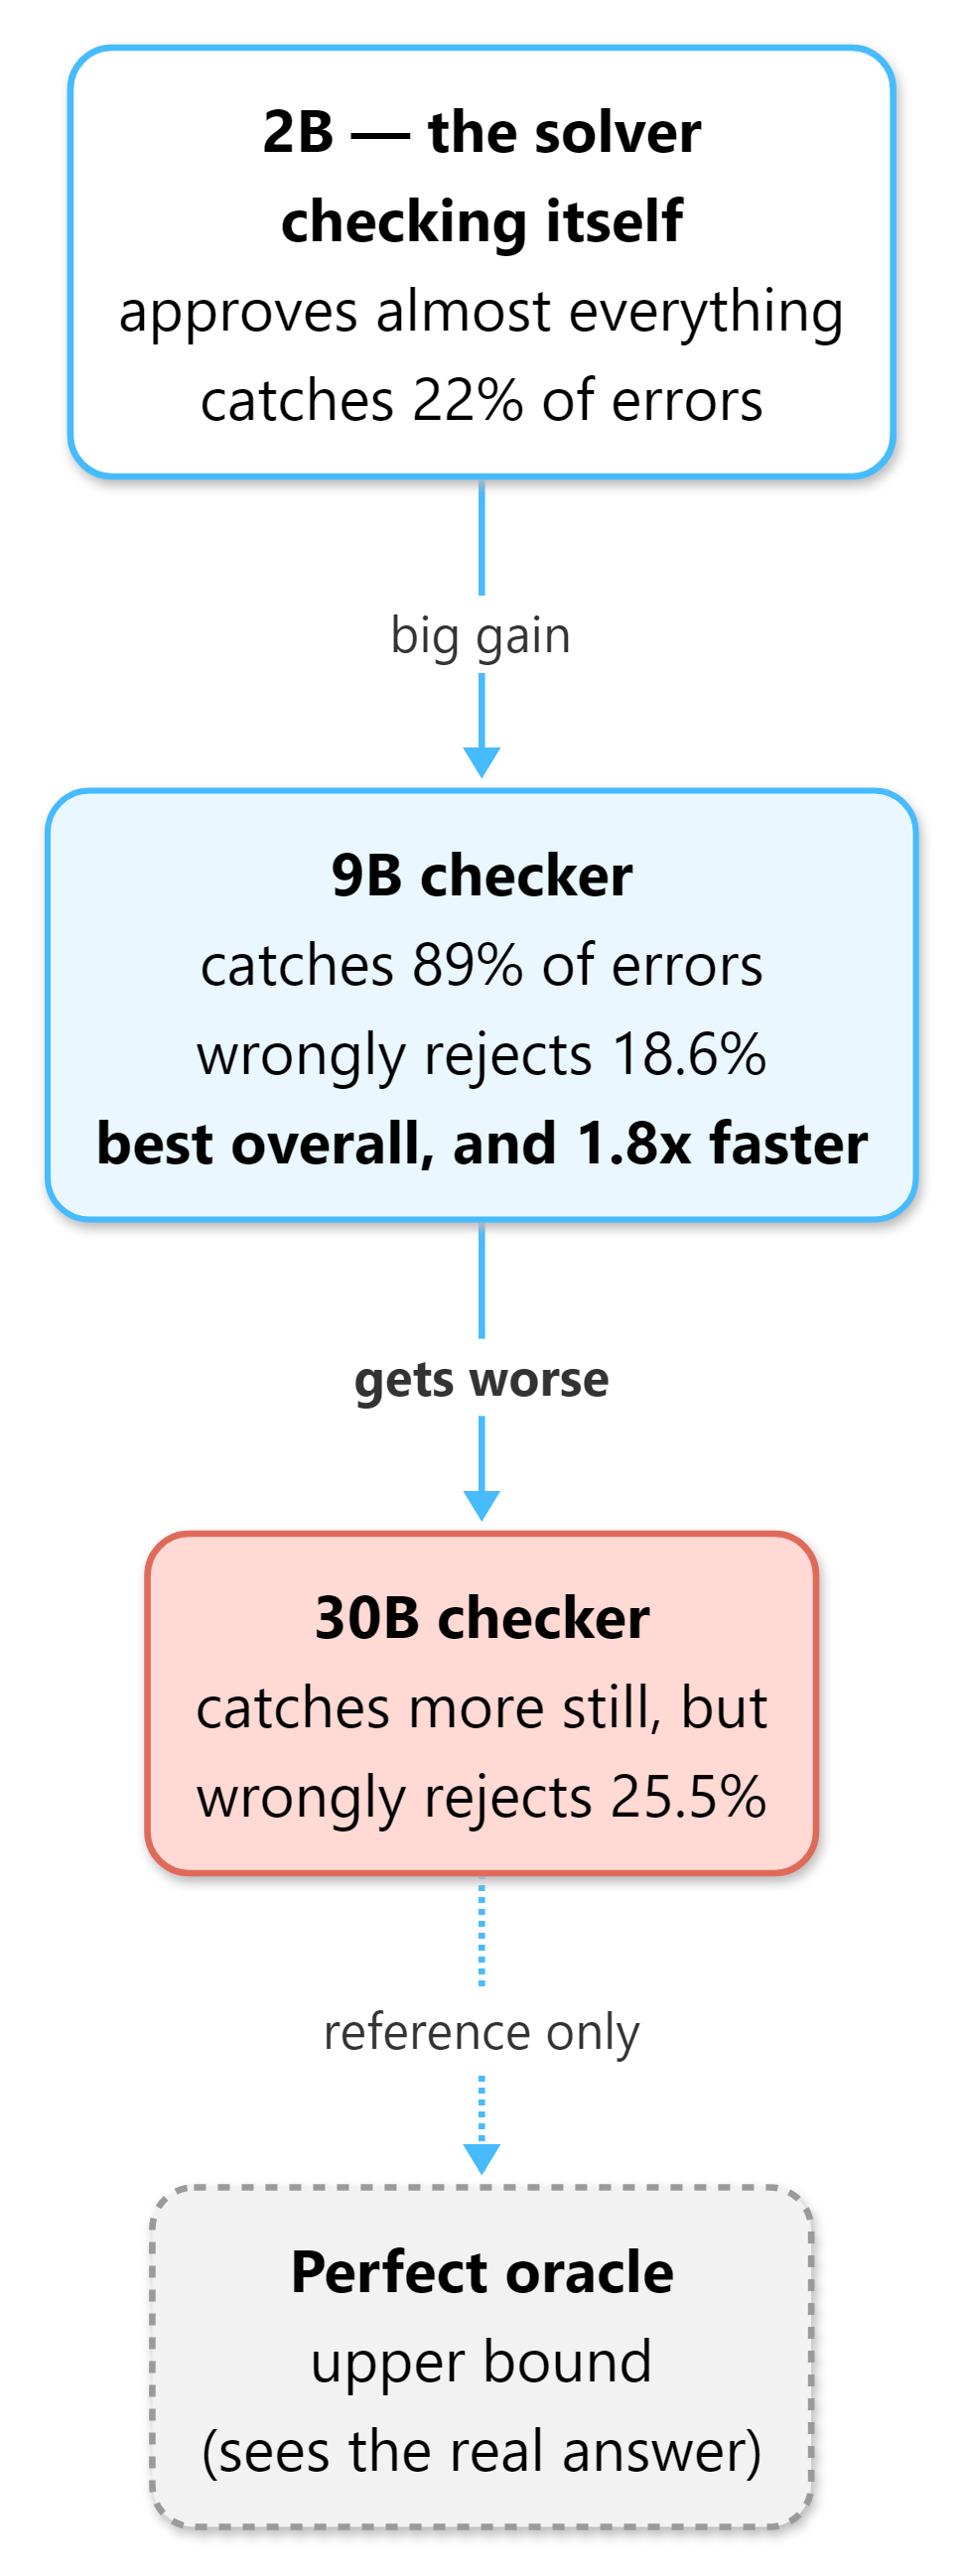
\includegraphics[width=\columnwidth]{fig6_checker_strength_ladder.png}
\caption{Supervisor capability is not monotonically beneficial: the 9B verifier dominates
the 30B one on every measure taken.}
\label{fig:ladder}
\end{figure}

\begin{table}[t]
\caption{The verifier ladder.}
\label{tab:ladder}
\centering
\small
\begin{tabular}{@{}lccccr@{}}
\toprule
Verifier & Size & Recall & False-rej. & Prec. & s/judg. \\
\midrule
Self-verification & 2B & 0.22 & 0.42 & 0.44 & 13.0 \\
\textbf{Qwen3.5-9B} & 9B & \textbf{0.888} & \textbf{0.186} & \textbf{0.791} & \textbf{1.00} \\
GLM-4.7-Flash & 30B-A3B & 0.835 & 0.255 & 0.721 & 2.07 \\
Exact oracle & --- & 1.000 & 0.000 & 1.000 & --- \\
\bottomrule
\end{tabular}
\end{table}

\textbf{Self-verification fails comprehensively.} The 2B solver judging its own work caught
$22\%$ of errors, wrongly rejected $42\%$ of correct answers, and produced unparseable
output on 19 of 30 trials. It was also $6\times$ slower per judgment than the 30B model ---
serving stack and active parameter count dominate total parameter count. This is the
behaviour self-enhancement bias~\cite{zheng2023judge} predicts.

\textbf{The 9B verifier dominates the 30B one} on recall ($+31$ errors caught),
false-reject rate ($-51$ correct answers broken) and precision, at half the latency and a
third of the file size (5.6\,GB against 16.3\,GB). Given the resampling asymmetry of
Section~\ref{sec:free}, the false-reject column is the expensive one: a larger verifier
more willing to find fault with correct reasoning is not more careful, it is more costly.
There appears to be a verifier scale suited to this task, and 30B overshoots it. The 2B row
is a 30-question preflight, not a full pass; Section~\ref{sec:limits} explains why we now
treat preflights as budget decisions only.

\subsection{The full system}
\label{sec:full}

\begin{table}[t]
\caption{Accuracy against off-device cost.}
\label{tab:full}
\centering
\small
\begin{tabular}{@{}lrrrr@{}}
\toprule
Configuration & Corr. & Acc. & Tok./q & Calls \\
\midrule
Fine-tuned solver & 737 & $55.88\%$ & 0.0 & 0 \\
Self-consistency@3 & 779 & $59.06\%$ & 0.0 & 0 \\
GLM cascade, un-stacked & 784 & $59.44\%$ & 296.0 & 712 \\
GLM cascade, stacked & 826 & $62.62\%$ & 296.0 & 712 \\
GLM @ $37.3\%$, stacked & 843 & $63.91\%$ & 369.0 & 889 \\
GLM combined gate, stacked & 837 & $63.46\%$ & 307.5 & 728 \\
Qwen cascade, un-stacked & 861 & $65.28\%$ & 345.8 & 728 \\
\textbf{Qwen combined, stacked} & \textbf{903} & $\mathbf{68.46\%}$ & \textbf{345.8} & \textbf{728} \\
\textit{pass@3 ceiling} & \textit{962} & \textit{$72.93\%$} & --- & --- \\
\bottomrule
\end{tabular}
\end{table}

% ---------------------------------------------------------------------------
% FIGURE 6  *** the headline chart ***
% REPLACE WITH: nothing, unless you want it restyled.
%   Current source : reports/figures/pareto.pdf  (a real vector PDF -- prefer
%                    this over the .png for print quality)
%   Generated by   : experiments/plot_pareto.py, directly from
%                    reports/fydp3_summary.csv
%   A dumbbell chart, not a scatter. One row per configuration; the pale marker
%   is the arm run instead of the vote, the dark one the same run stacked on it.
%   If redrawn, keep the pairing -- the gap IS the result.
%   FULL WIDTH (figure*): at \columnwidth its labels fall to about 5pt.
%   Save as figures/pareto.pdf.
% ---------------------------------------------------------------------------
\begin{figure*}[t]
\centering
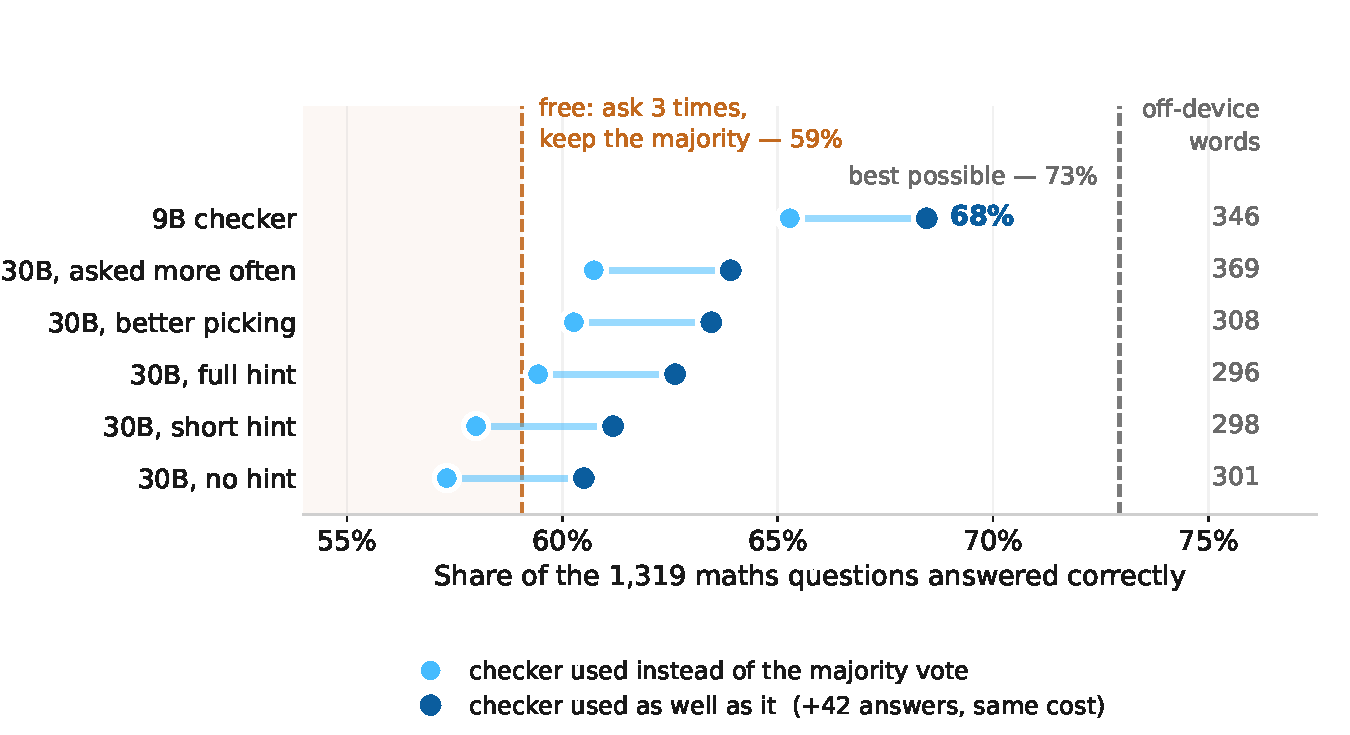
\includegraphics[width=0.88\textwidth]{pareto.pdf}
\caption{Every supervised configuration, best first. Each is scored twice: the light marker is
the checker used \emph{instead of} the majority vote, the dark marker the identical run
\emph{stacked on} it. Every pair differs by exactly $+42$ answers at identical cost. Off-device
cost is given in the right-hand column rather than as a second axis. The fine-tuned model
alone, not shown, scores $55.88\%$.}
\label{fig:pareto}
\end{figure*}

The best configuration reaches $68.46\%$ --- $93.9\%$ of the pass@3 ceiling --- with $70\%$
of questions resolved entirely on-device and a mean of $345.8$ off-device tokens per
question across the whole test set.

\textbf{The stacking effect.} Every stacked arm gains exactly $+42$ answers over its
un-stacked counterpart at identical cost: $756\rightarrow798$, $765\rightarrow807$,
$784\rightarrow826$, $801\rightarrow843$, $795\rightarrow837$. The invariance is the
structural property predicted in Section~\ref{sec:stacking} --- voting and escalation
operate on disjoint buckets --- and not a tuned quantity.

\textbf{Feedback level.} Holding everything else fixed, richer hints help monotonically:
L0 $57.32\%$, L1 $58.00\%$, L2 $59.44\%$ un-stacked. L2 costs $5.5\times$ L0's output
tokens for $+2.1$ points. All three arms rejected an identical question set, by the caching
control of Section~\ref{sec:cache}.

\subsection{Significance}

Both systems answer identical questions, so we use \emph{exact} McNemar on the discordant
pairs --- the exact binomial rather than the $\chi^2$ approximation, since several
discordant counts are small.

\begin{table}[t]
\caption{Significance (McNemar, exact) against two controls.}
\label{tab:sig}
\centering
\small
\begin{tabular}{@{}lcc@{}}
\toprule
Configuration & vs. baseline ($p$) & vs. self-cons. ($p$) \\
\midrule
Cascade only, GLM-30B & $<0.001$ & $\mathbf{0.247}$ \\
Cascade + voting, GLM-30B & $<0.001$ & $<0.001$ \\
Cascade only, Qwen-9B & $<0.001$ & $<0.001$ \\
Cascade + voting, Qwen-9B & $<0.001$ & $<0.001$ \\
\bottomrule
\end{tabular}
\end{table}

The second column is the one that matters, and row 1 is the result we consider most
important to report. Against free self-consistency, \emph{no un-stacked GLM configuration
is distinguishable} --- $p=0.062$, $0.275$, $0.751$, $0.127$ and $0.247$ for the five arms.
As configured, that cascade is not justified over majority voting despite 712 supervisor
calls.

Two independent remedies recover the result. Stacking moves every arm to significance
(e.g.\ 23 vs.\ 70 discordant, $p<0.001$). And changing the verifier does so even without
stacking: the un-stacked Qwen arm reaches $65.28\%$ against $59.06\%$, 148 vs.\ 66
discordant, $p<0.001$. The original null was a property of the verifier, not of the design.

The best system flips 190 answers wrong$\rightarrow$right against 24
right$\rightarrow$wrong --- the most favourable ratio of any configuration tested, and a
direct consequence of the 9B verifier's lower false-reject rate.

\subsection{Latency, and a correction to the cost argument}

\begin{table}[t]
\caption{Measured latency ($n=40$ questions).}
\label{tab:latency}
\centering
\small
\begin{tabular}{@{}lr@{}}
\toprule
Operation & Mean \\
\midrule
Local solution generation & 15.12\,s \\
Qwen3.5-9B judgment & 1.00\,s \\
GLM-4.7-Flash judgment & 2.07\,s \\
On-device path (composed) & 45.37\,s \\
Escalated path (composed) & 59.05\,s \\
\textbf{Mean across all questions} & \textbf{49.47\,s} \\
\bottomrule
\end{tabular}
\end{table}

The composed system is $3.3\times$ slower than a single answer. The breakdown reframes the
argument: generating three local samples accounts for $91.7\%$ of the time, the retry
$7.7\%$, and waiting on the supervisor $0.6\%$.

We state the consequence plainly. \textbf{Rare escalation is justified by data locality and
monetary cost, not by latency.} The expense is the gate's sampling, which is local. A
reader should not take ``the cascade is fast'' from this work. Note also that the 2B solver
through \texttt{transformers} is $15\times$ slower per token than the 9B supervisor through
\texttt{llama.cpp}, which suggests the largest available speed improvement is a serving
change rather than a modelling one. These figures come from a desktop GPU, not the
deployment target, and should be read as a lower bound.

% ============================================================================
\section{Discussion}
% ============================================================================

\subsection{The obvious design does not work}

Our first complete system escalated $30\%$ of questions to a 30B supervisor with full hints
and reached $59.44\%$, against $59.06\%$ for majority voting at zero off-device cost,
$p=0.751$. Five answers, for 712 supervisor calls.

The error was treating voting and verification as alternatives. They repair disjoint
question sets: voting resolves the bucket where a majority exists, verification operates
where no majority exists. Because the gate already samples three times, the vote is
available at no additional cost, and discarding it is a pure loss. Stacking recovers $+42$
answers at identical expenditure. We consider this the most transferable finding in the
paper, because it is the mistake a reader implementing a cascade over a small model is most
likely to repeat.

\subsection{Bigger verifiers are not better verifiers}

The 9B model dominates the 30B on every measured axis. We attribute this to the asymmetry
established in Section~\ref{sec:free}: because resampling breaks correct answers more often
than it repairs incorrect ones, every false rejection is a negative-expectation gamble. A
larger model more inclined to find fault in valid reasoning converts that inclination
directly into lost accuracy. Verifier selection should therefore optimise false-reject
rate, not capability in the abstract --- and the 5.6\,GB verifier is also the one that fits
alongside the solver.

\subsection{The first failure was the verifier's}

The null against self-consistency did not survive the verifier change: the un-stacked Qwen
configuration beats voting at $p<0.001$. The cascade design was sound throughout; it was
being evaluated with a verifier whose false-reject rate consumed the gain. This is a
caution about generalising from a single verifier --- a negative result for a cascade may be
a negative result for one judge.

% ============================================================================
\section{Limitations}
\label{sec:limits}
% ============================================================================

\begin{enumerate}
\item \textbf{The pass@3 ceiling ($72.93\%$) bounds everything.} No verifier can recover an
answer the solver never generated.
\item \textbf{We verify final answers, not reasoning.} No claim is made that solutions are
correct for the right reasons; the hand-labelled study that would establish this was not
performed.
\item \textbf{Retries are not reproducible per question.} Aggregate accuracy is stable
($0.3232$ vs.\ $0.3308$ on the shared set, $p=0.826$) but only $32\%$ of individual final
answers were identical across runs. Our results are reproducible as rates, not as
per-question outcomes.
\item \textbf{Effects below roughly 40 answers are undetectable} at $n=1{,}319$. The
combined gate's $+11$ ($p=0.343$) lies inside that band; we report it as a cost saving
($17\%$ fewer off-device tokens) rather than an accuracy claim.
\item \textbf{Anchoring.} The retry prompt contains the rejected solution, risking
repetition of the original error. We observed this qualitatively but did not quantify it.
\item \textbf{The self-verification row is 30 questions.} A 30-question preflight put the
9B verifier's false-reject rate at $0.417$; the full pass measured $0.186$, reversing the
recommendation and nearly causing us to discard our best verifier. Part of the cause was
mechanical --- a 200-token reply cap truncated a model that writes longer replies. The rule
we adopted: a preflight decides whether to spend the GPU time; it never decides what to
conclude.
\item \textbf{The stacking hypothesis was formed after observing test results.} It was not
pre-registered. We disclose this rather than present it as planned.
\item \textbf{Verifiers are not bit-reproducible}, which the verdict cache controls for
within our comparisons but which remains a property of the tooling.
\item \textbf{All latency is from a desktop GPU}, not from the constrained hardware the
design targets.
\item \textbf{Our best score is slightly understated.} The 9B verifier truncated 50 of 728
replies ($6.9\%$); 8 of those waved through incorrect answers, worth roughly 2 answers.
\item \textbf{One solver, one dataset.} The gate, tie-break and stacking behaviours are
demonstrated on \texttt{gemma-4-E2B-it} on GSM8K. This is the most substantial open
question in the work. The mechanism is shown to work; its generality is future work.
\item \textbf{GSM8K is a controlled probe, not a workload.} It was selected for automatic,
unambiguous grading, not because grade-school arithmetic on-device is a pressing need.
\end{enumerate}

% ============================================================================
\section{Conclusion}
% ============================================================================

We built and measured an edge-constrained supervised cascade for grade-school mathematical
reasoning. A 4-bit 2B solver fine-tuned with QLoRA reaches $55.88\%$ on GSM8K; adding a
self-consistency vote, a free disagreement gate, and a 9B supervisor consulted on $30\%$ of
questions reaches $68.46\%$, or $93.9\%$ of the pass@3 ceiling, with $70\%$ of questions
resolved entirely on-device.

Three findings we would defend. A supervised cascade must be \emph{stacked on}
self-consistency rather than substituted for it: substituted, ours was statistically
indistinguishable from free voting; stacked, every arm gained exactly $+42$ answers at
identical cost. Verifier capability is not monotonic in size --- a 9B verifier dominated a
30B one on every measure while running twice as fast. And the strongest gate signal is free
when voting is already in use, since sample disagreement (AUC $0.840$) outperforms
single-pass confidence ($0.715$), with a lexicographic tie-break reaching $0.869$ without
introducing a tunable weight.

Future work, in order of expected value: serve the solver through the same optimised runtime
as the supervisor, since $91.7\%$ of latency is local sampling and the supervisor is
$15\times$ faster per token; test whether the gate and stacking behaviours transfer to a
different solver; measure on the constrained hardware the design targets; and hand-label a
reasoning sample to close Limitation 2.

% ============================================================================
\bibliographystyle{IEEEtran}
\bibliography{references}

\end{document}
